The Scenario Co-Evolution method by Gabor et al. \cite{gabor19} is another novel approach to tackle the issue of testing learning systems reliably. If not stated otherwise the content of this chapter derives from the original publication.\\
This concept is an instance of the general architecture of \cite{gabor18} briefly mentioned in section \ref{limitations}. The basic idea is to train an evolutionary algorithm, that co-evolves with a reinforcement learning agent and actively finds problems that are hard to solve for the agent. While the expertise of the agent evolves, the set of test instances (or \textit{scenarios}) co-evolves. After training, the co-evolutionary algorithm should return a set of hard test scenarios, that can be used for evaluating the agent.\\\\
More specifically, hard settings $x$ (or values $x$) from the scenario space $\chi$, for which the agents' performance deteriorates are wanted. Similar to Zero-sum Markov games (section \ref{zerosumgames}) two algorithms optimize against each other. While the agent tries to maximize its fitness, the co-evolutionary algorithm tries to find scenarios which minimize the agents' fitness. An evolutionary algorithm (section \ref{evolutionaryalgorithms}) that optimizes for hard settings for $x$ is used to find those the respective values for $x$. Figure \ref{fig:scenario_coevolution} shows a visual representation of the evolutionary algorithm.
\begin{figure}
  \centering
  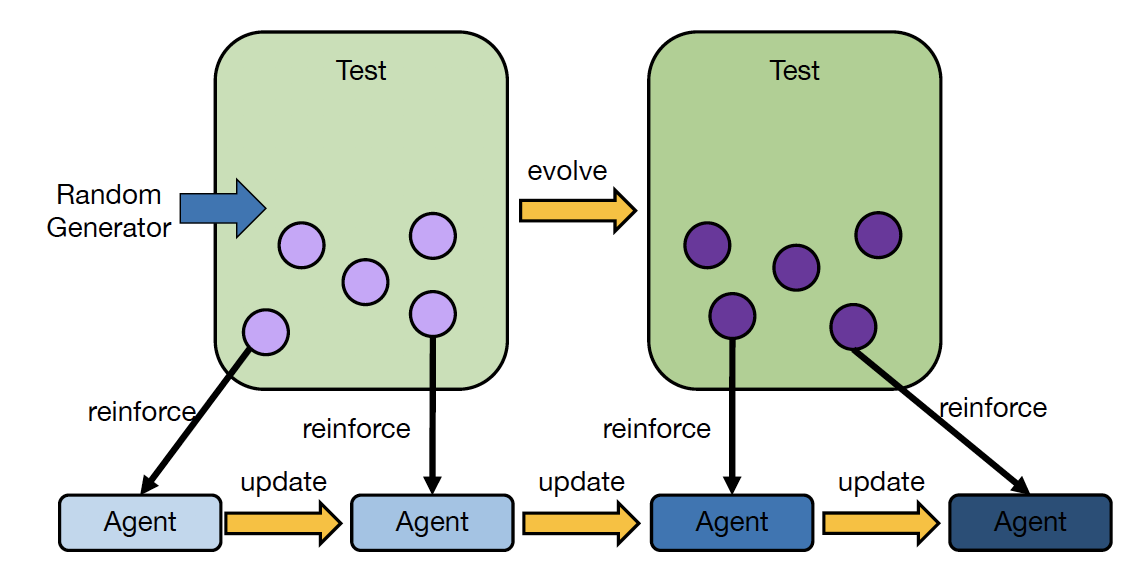
\includegraphics[width=0.85\textwidth]{adversarial_learning/images/scenario_coevolution.png}
  \label{fig:scenario_coevolution}
  \caption{Visual representation of the evolutionary process by \cite{gabor19}. First, a set of test scenarios is randomly generated. The set improves via evolution. Between evolution steps, the test data is used to train the agent. This causes the reinforcement learning agent to co-evolve with the test data.}
\end{figure}
It constructs an evolutionary process with the scenario space $\chi$. The experience samples necessary to train the agent are drawn using settings for $x \in \chi$ that are included in the current population $\chi$ of the evolutionary process. When all $x \in \chi$ have been used, the evolutionary process evolves further for a few generations. In this work, the evolutionary step function for selection schemes $\sigma_1, \sigma_2, \sigma_3$ is:
\begin{equation}
X_{i+1} = o(X_i) = sel(mig_{\sigma_3}(mut_{\sigma_2}(rec_{\sigma_1}(X_i))),|X_i|)
\end{equation}
After a few generations of optimizing for hard $x$ the resulting experience sample is used to generate experience samples for the reinforcement learning agent. As mentioned, the reinforcement learning agent tries to maximize its reward, while the evolutionary process tries to minimize the fitness. The fitness $f(x)$ assigned to each $x \in \chi$ is computed using the accumulated reward of running the current agent policy $\pi$ on the MDP $M_x$ (section \ref{mdp}).
In turn, the reinforcement learning agent with the current highest fitness score is used to evaluate the hardness of the settings for $x$ for the next few generations of evolution.\\
With every evolutionary step the agent trains on harder settings from the test population. Simultaneously the fittest agent evaluates the hardness of the settings. In the end, the algorithm is able to return a set with the hardest test scenarios. When the agent can solve these hard problems, it can be assumed that it can solve easy scenarios, too. Consequently, there is no need to generate all possible scenarios. Additionally, these scenarios are not limited to the trained agent. They can be used to evaluate every agent running on the same environment.